\documentclass[t,handout]{beamer}
\usepackage[utf8]{inputenc}
\usepackage[ngermanb]{babel}
\usepackage{listings}
\lstset{basicstyle=\tiny}
% \lstset{language=bash}
\definecolor{darkblue}{rgb}{0,0,.5}
\hypersetup{pdftex=true, colorlinks=true, breaklinks=true, linkcolor=darkblue, menucolor=darkblue, pagecolor=darkblue, urlcolor=darkblue}

\title{Taskwarrior -- What's next?}
\subtitle{Task management on the commandline}
% \author[Deimeke, Dirk]{Dirk Deimeke}
\author{Dirk Deimeke}
% \institute[Ubucon 2011]{Deutsche Ubuntu Konferenz 2011}
\institute{OpenRheinRuhr 2011}
% \date[16.10.2011]{16. Oktober 2011}
\date{November 2011}
\titlegraphic{
\includegraphics[width=3cm,height=3cm]{tw-xxl}}
\subject{Taskwarrior}
\keywords{taskwarrior, task, management, commandline, getting things done}

\setbeamercovered{transparent}

\pgfdeclareimage[width=5mm]{tw-logo}{tw-xl}

%%%%%%%%%%%%%%%%%%%%%%%%%%%%%%%%%%%%%%%%%%%%%%%%%%%%%%%%%%%%%%%%%%%%%%%
%
% LaTeX-Template for Taskwarrior by Dominik Wagenführ
% http://www.deesaster.org/
%
% Creative Commons Attribution-ShareAlike 4.0 (CC-BY-SA 4.0)
% https://creativecommons.org/licenses/by-sa/4.0/
%
%%%%%%%%%%%%%%%%%%%%%%%%%%%%%%%%%%%%%%%%%%%%%%%%%%%%%%%%%%%%%%%%%%%%%%%

%%%%%%%%%%%%%%%%%%%%%%%%%%%
% Layout - Start
%%%%%%%%%%%%%%%%%%%%%%%%%%%

\setbeamertemplate{navigation symbols}{}

\useinnertheme{default}
\useoutertheme{infolines}
\usefonttheme{structurebold}

\newlength{\boxwidth}
\setlength{\boxwidth}{121px}
\setbeamertemplate{headline}{%
\begin{beamercolorbox}[dp=3px,ht=6px,wd=\boxwidth,center]{palette tertiary}%
\insertauthor\ (\insertinstitute)%
\end{beamercolorbox}%
\vskip-9px\hskip\boxwidth
\begin{beamercolorbox}[dp=3px,ht=6px,wd=\boxwidth,center]{palette secondary}%
\inserttitle%
\end{beamercolorbox}%
\begin{beamercolorbox}[dp=3px,ht=6px,wd=\boxwidth,right]{palette primary}%
\insertdate\hskip15px\insertframenumber\,/\,\inserttotalframenumber\hspace*{8px}
\end{beamercolorbox}%
}
\setbeamertemplate{footline}{}

%%%%%%%%%%%%%%%%%%%%%%%%%%%
% Colors - Start
%%%%%%%%%%%%%%%%%%%%%%%%%%%

\definecolor{basecolor}{gray}{0.2}
\definecolor{mittelgrau}{gray}{0.4}
\definecolor{hellgrau}{gray}{0.93}
\definecolor{gelb}{rgb}{1.0,1.0,0.75}

% infolines color
\setbeamercolor{palette primary}{fg=white,bg=mittelgrau}
\setbeamercolor{palette secondary}{fg=white,bg=basecolor}
\setbeamercolor{palette tertiary}{fg=white,bg=black}

% frame and title color
\setbeamercolor{frametitle}{fg=white,bg=basecolor}
\setbeamercolor{titlelike}{fg=white,bg=basecolor}
\setbeamerfont{frametitle}{series=\bfseries}

% TOC color
\setbeamercolor{section in toc}{fg=basecolor}

% text color
\setbeamercolor{normal text}{fg=black,bg=white}

% item color
\setbeamercolor{item}{fg=basecolor}
\setbeamercolor{itemize item}{fg=black}

% block color
\setbeamercolor{block title}{fg=black,bg=gelb}
\setbeamercolor{block body}{fg=black,bg=gelb}

% block alert color
\setbeamercolor{block title alerted}{fg=black,bg=gelb}
\setbeamercolor{block body alerted}{fg=black,bg=gelb}

% block example color
\setbeamercolor{block title example}{fg=black,bg=gelb}
\setbeamercolor{block body example}{fg=black,bg=gelb}

\setbeamertemplate{frametitle}{%
\vskip-1px%
\begin{beamercolorbox}[wd=363px,ht=20px,dp=12px]{frametitle}
\usebeamerfont{frametitle}%
\usebeamercolor{frametitle}%
\vspace*{-5px}\hspace*{10px}
\includegraphics[width=24px,height=24px]{tw-xl.png}\\
\vspace*{-20px}\hspace*{40px}\insertframetitle%
\end{beamercolorbox}
}

%%%%%%%%%%%%%%%%%%%%%%%%%%%
% Colors - Stop
%%%%%%%%%%%%%%%%%%%%%%%%%%%

%%%%%%%%%%%%%%%%%%%%%%%%%%%%%%%%%%%%%%%%%%%%%%%%%%%%%%%%%%%%%%%%%%%%%%%

\begin{document}

\frame{\titlepage}

% \logo{\pgfuseimage{tw-logo}}

% \frame{\frametitle{Content}\tableofcontents}

\section{Introduction} 
\parskip1ex

\frame{\frametitle{Dirk Deimeke (that's me)}
\begin{itemize}
	\item Maried, two dogs
	\item Born in Wanne-Eickel
	\item Living in Grüt (2008 emigrated to Switzerland)
	\item Senior Unix Systems Administrator in Zürich
	\item More \url{http://d5e.org/}
\end{itemize}
}

\frame{\frametitle{Dirk Deimeke (Taskwarrior)}
\begin{itemize}
	\item I first saw Taskwarrior at Ubucon 2009 in a lightning talk of \href{http://f.ederi.co/}{Federico Hernandez}, one of the core developers. \pause
	\item Started to use it in the beginning of 2010. \pause
	\item Still enthusiastic about it! ;-) \pause
	\item In the middle of 2010 I joined the \href{http://taskwarrior.org/wiki/Credits}{Taskwarrior Core Team}
	\item I like working in an international team
	\begin{itemize}
		\item Watertown (Massachusetts, USA)
		\item Gothenburg (West Gothland, Sweden)
		\item Braunschweig, (Lower Saxony, Germany)
		\item Richmond (Virginia, USA)
		\item Bonn (North Rhine-Westphalia, Germany)
		\item Toronto (Ontario, Canada)
		\item Gruet (Zurich, Switzerland)
	\end{itemize}
	\item \url{http://taskwarrior.org/}
	\item \url{http://d5e.org/taskwarrior} (German) own blog-articles
\end{itemize}
}

\frame{\frametitle{About this session}
\begin{itemize}
\item \textbf{What is this all about?} \\
This is about Taskwarrior, an efficient tool for task management. Techniques for time management are not part of this session. \pause 
\item \textbf{Why do you use the beta-Version?} \\
With Taskwarrior 2.0.0 a new syntax will be introduced and it makes no sense to show the old commands. \pause
\end{itemize}

\begin{alertblock}{Attention!}
\begin{itemize}
    \item Feel free to ask any questions!
    \item If you find any errors, please tell me.
\end{itemize}
\end{alertblock}
}

\frame{\frametitle{Project founder: Paul Beckingham}
\pause
\begin{itemize}
\item I started out using Gina Trapani's todo.sh, which was great, but I soon wanted features that would have been difficult to implement in a shell script, so I wrote my own. \pause
\item It stemmed from the fact that a todo program needs to be simple to use, and unobtrusive, otherwise it's a hassle. But it can't be too simple. \pause
\item If you go to the trouble of capturing this information, it seems wasteful not to leverage it.  So it has a lot of features, but tries to remain simple to use. \pause
\item There are many different methodologies people use for managing their work, and taskwarrior tries to walk a line through the middle of all that, with features for all the different approaches. \pause
\item Taskwarrior is intended to scale with the user, from very simple straightforward usage up to quite sophisticated task management.
\end{itemize}
}

\frame{\frametitle{Reasons for Taskwarrior}
Taskwarrior
\begin{itemize}
	\item is easy to learn.
	\item grows along with the work.
	\item is unbelievably powerful.
	\item is very fast.
	\item is easily extensible. 
	\item is platform independent:
	\begin{itemize}
		\item Most flavours of Unix and Linux, including Mac OS X
		\item Windows with Cygwin
		\item via SSH from my mobile
		\item \url{http://taskwarrior.org/w/Platforms}
	\end{itemize}
	\item is actively developed.
	\item can be influenced by users (feature requests).
	\item has excellent and very friendly support.
\end{itemize}
}

\section{Installation}

\begin{frame}
\frametitle{5 steps to install from source}

All you need to compile is \texttt{gcc}, \texttt{cmake} and \texttt{make}. \pause

\begin{enumerate}
\item \href{http://taskwarrior.org/download}{Download} of recent version
\item \texttt{tar xzf task-2.0.0.beta4.tar.gz}
\item \texttt{cmake .} (not \texttt{./configure}!)
\item \texttt{make}
\item \texttt{sudo make install}
\end{enumerate}
\end{frame}

\begin{frame}[fragile]
\frametitle{Test of your installation}
\begin{lstlisting}
$ task version
A configuration file could not be found in /home/user

Would you like a sample /home/user/.taskrc created, so taskwarrior can proceed? (yes/no) yes

task 2.0.0.beta4 built for linux
Copyright (C) 2006 - 2011 P. Beckingham, F. Hernandez.

Taskwarrior may be copied only under the terms of the MIT license, which may be
found in the taskwarrior source kit.

Documentation for taskwarrior can be found using 'man task', 'man taskrc', 'man
task-tutorial', 'man task-color', 'man task-sync', 'man task-faq' or at
http://taskwarrior.org

\end{lstlisting}
\end{frame}

\section{Simple ToDo-Lists}

\begin{frame}
\frametitle{A simple example, part 1}
\begin{center}
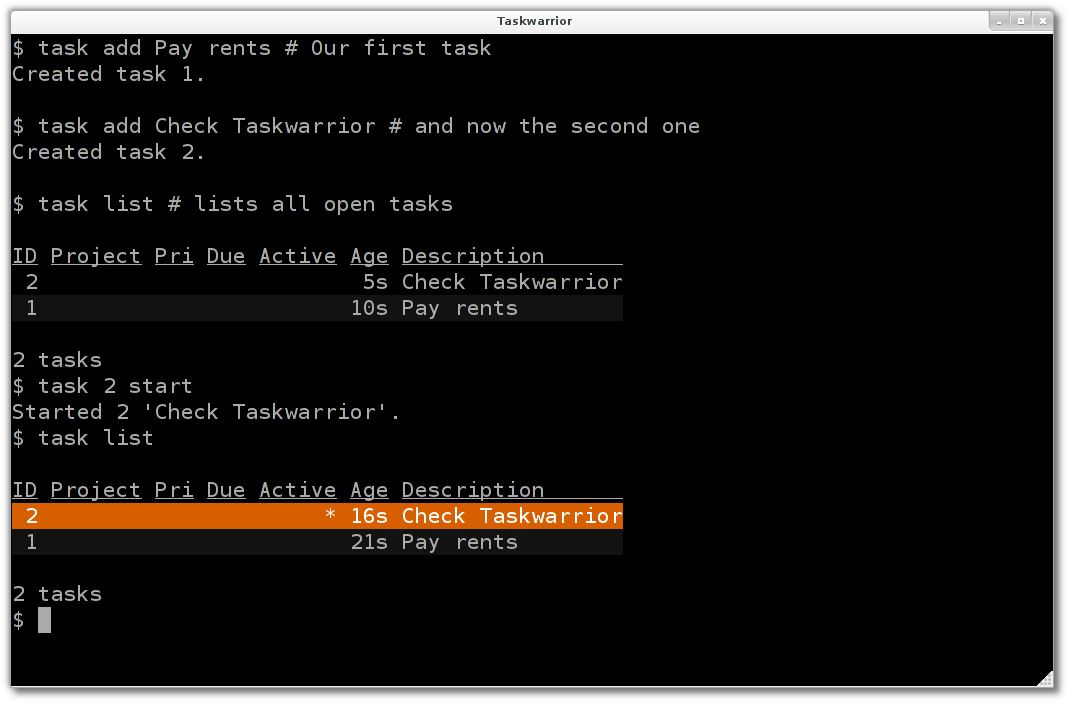
\includegraphics[width=10cm,height=7.5cm]{simple_example01.png}
\end{center}
\end{frame}

\begin{frame}
\frametitle{A simple example, part 2}
\begin{center}
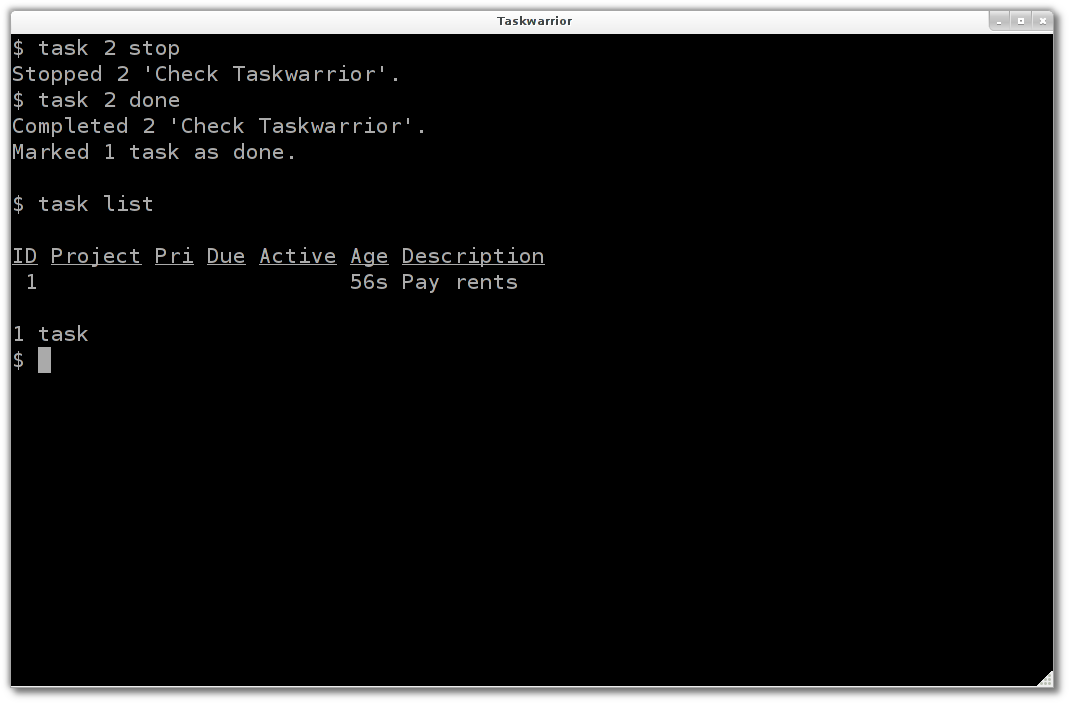
\includegraphics[width=10cm,height=7.5cm]{simple_example02.png}
\end{center}
\end{frame}

\begin{frame}
\frametitle{Commands so far}
\begin{itemize}
\item \textbf{task add} \\
Adds a new task to the task list. \pause
\item \textbf{task list} \\
Provides a standard listing of tasks. \pause
\item \textbf{task start} \\
Marks the specified tasks as started. \pause
\item \textbf{task stop} \\
Removes the start time from the specified task. \pause
\item \textbf{task done} \\
Marks the specified task as done.
\end{itemize}
\end{frame}

\frame{\frametitle{That's it!}
\begin{center}
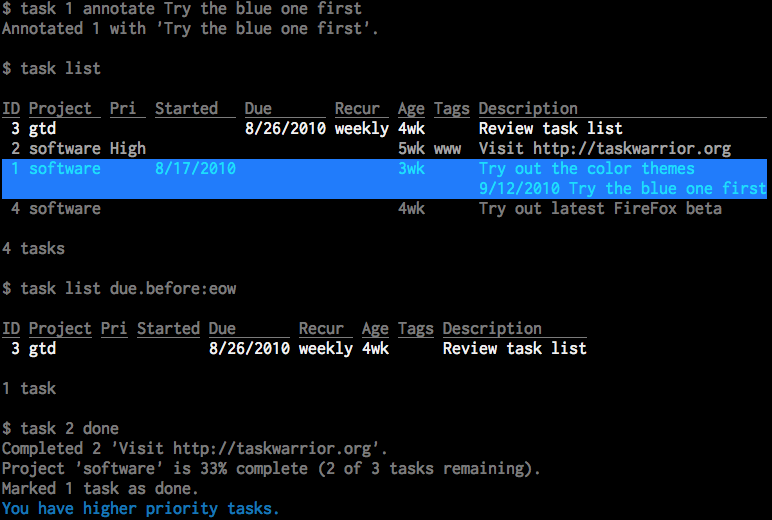
\includegraphics[width=6cm,height=4.5cm]{default-large.png}

\huge{Thanks for your attention!}

\normalsize{\href{mailto:dirk@deimeke.net}{dirk@deimeke.net}}

\url{http://taskwarrior.org/}
\end{center}
}

\section{General}

\frame{\frametitle{Just kidding ...}
\textbf{There is a lot more to explore.}

Even the commands from the last section are more mighty than they seem. \pause

\begin{itemize}
\item \textbf{task add {\tt<}mods{\tt>}}
\item \textbf{task {\tt<}filter{\tt>} list}
\item \textbf{task {\tt<}filter{\tt>} start {\tt<}mods{\tt>}}
\item \textbf{task {\tt<}filter{\tt>} stop {\tt<}mods{\tt>}}
\item \textbf{task {\tt<}filter{\tt>} done {\tt<}mods{\tt>}}
\end{itemize} \pause

To get an overview, take a look at the \href{http://www.taskwarrior.org/download/task-2.0.0.ref.pdf}{cheat sheet} (pdf, 145kB).
}

\begin{frame}
\frametitle{task {\tt<}filter{\tt>} command {\tt<}mods{\tt>}}
\pause
\begin{itemize} 
\item Is the basic usage of all task related write commands. \pause
\item Write commands can operate on one task or a group of tasks or even on all tasks. \pause
\item Every command maybe abbreviated up to the minimum that is necessary to identify a single command. \pause
\item Filters can be anything from nothing to simple IDs further to regular expressions or Boolean constructs. \pause
\item Modifications can be either a change of description, a change of dates or anything else that changes a task. \pause
\item In our simple example we already used the write commands \textbf{add}, \textbf{done}, \textbf{start} and \textbf{stop}.
\end{itemize}
\end{frame}

\begin{frame}
\frametitle{Scripts}
\begin{center}
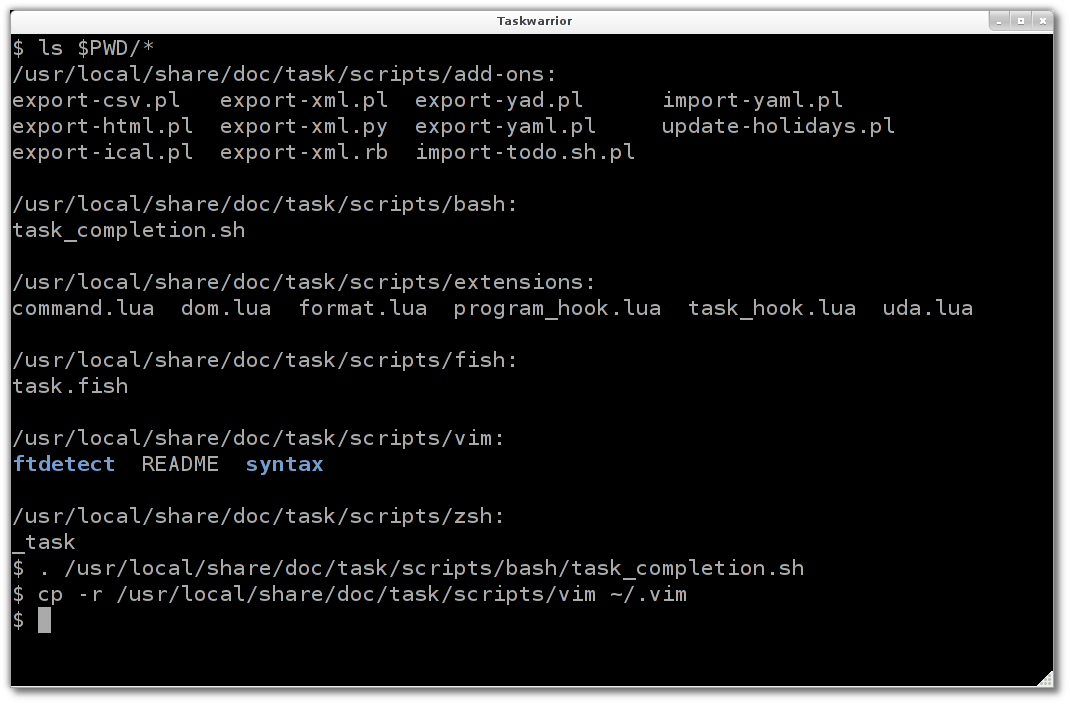
\includegraphics[width=10cm,height=7.5cm]{scripts.png}
\end{center}
\end{frame}

\begin{frame}
\frametitle{Most important commands}

These are the most important commands, just because I use them most ;-)

\begin{itemize}
\item \textbf{task {\tt<}filter{\tt>} modify} \\
The name says it, it modifies tasks according to the filter used. \pause
\item \textbf{task {\tt<}filter{\tt>} edit} \\
This starts your favourite editor with the tasks you want to change. \\
(Remember the syntax highlighting for vim?) \pause
\item \textbf{task undo} \\
Reverts the most recent change to a task. \pause
\item \textbf{task help} \\
Gives an overview of implemented commands and custom reports. \pause
\item \textbf{man task (taskrc, task-tutorial, task-color, task-faq, task-synch)} \\
Show the (almighty) man-page(s). Unlike the man-pages of many other 
programs they are extremely helpful and full of information and examples. 
Try them!
\end{itemize}
\end{frame}

\section{Working with dates}

\begin{frame}
\frametitle{Set dateformat (check "man taskrc")}
\begin{center}
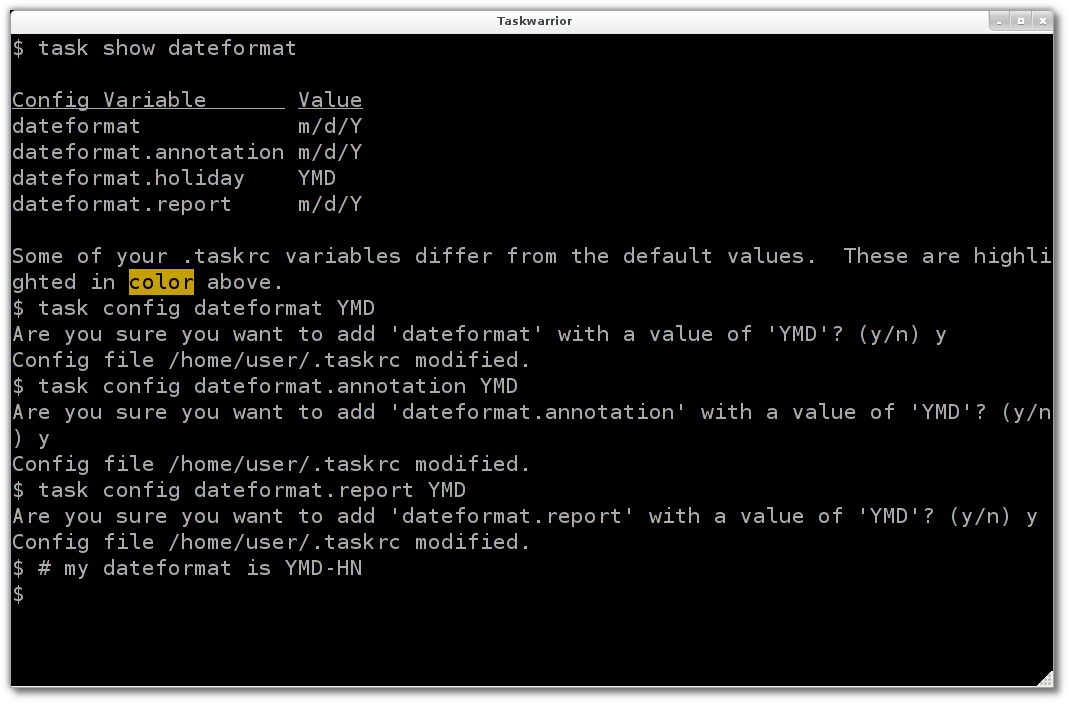
\includegraphics[width=10cm,height=7.5cm]{set_dateformat.png}
\end{center}
\end{frame}

\begin{frame}
\frametitle{Set weekstart}
\begin{center}
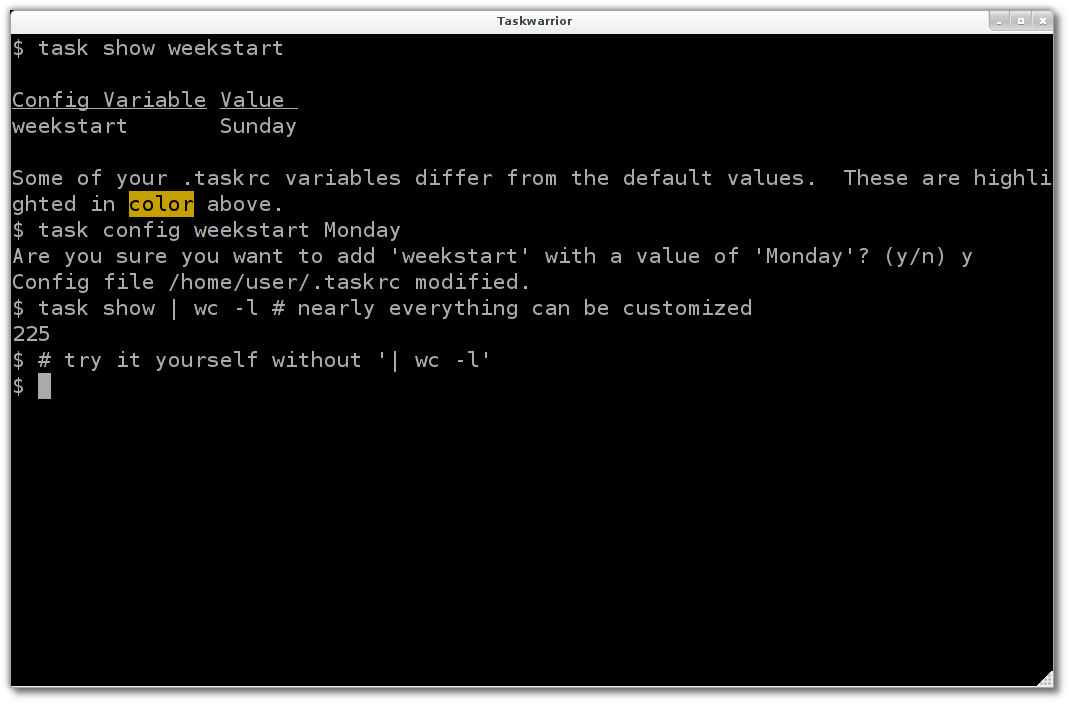
\includegraphics[width=10cm,height=7.5cm]{set_weekstart.png}
\end{center}
\end{frame}

\begin{frame}
\frametitle{Special dates}
\begin{itemize}
\item \textbf{Relative wording} \\ today, yesterday, tomorrow
\item \textbf{Day number with ordinal} \\ 23rd, 3wks, 1day, 9hrs
\item \textbf{At some point or later} \\ later, someday
\item \textbf{Start / end of (work) week, calendar week (according to settings of weekstart), month, quarter and year} \\ sow, eoww, socw, eom, soq, eoy
\item \textbf{Next occurring weekday} \\ mon, tue, ..., sat, sun
\end{itemize}
\end{frame}

\begin{frame}
\frametitle{Due and wait}
\begin{center}
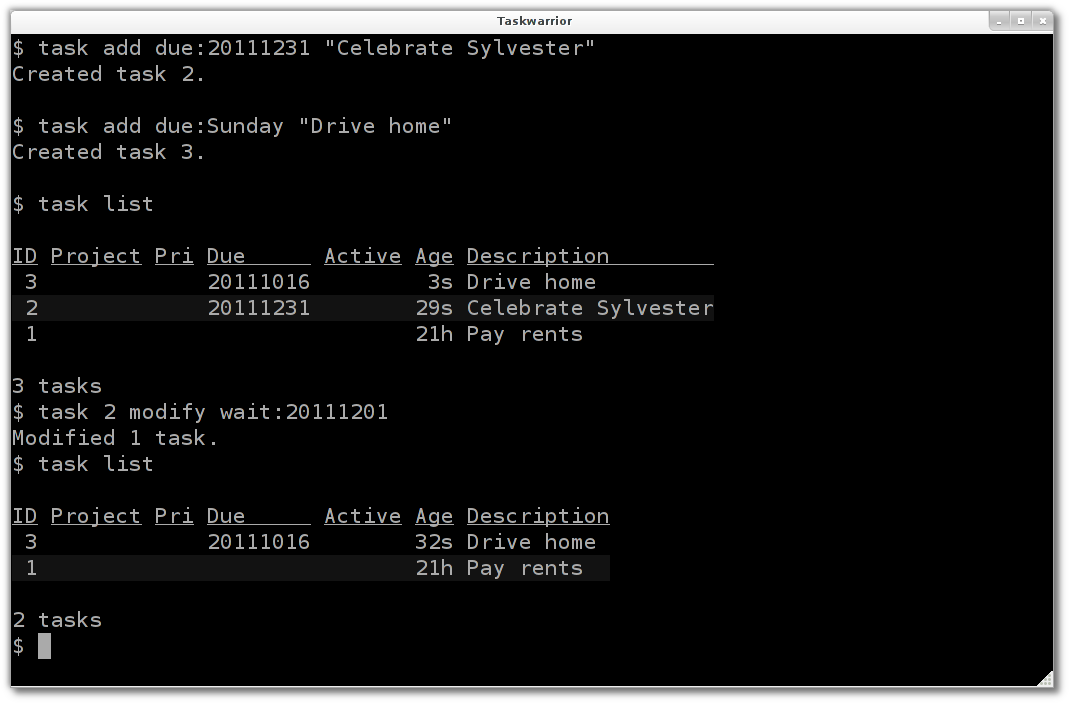
\includegraphics[width=10cm,height=7.5cm]{due_and_wait.png}
\end{center}
\end{frame}

\begin{frame}
\frametitle{Recurrence}
\begin{center}
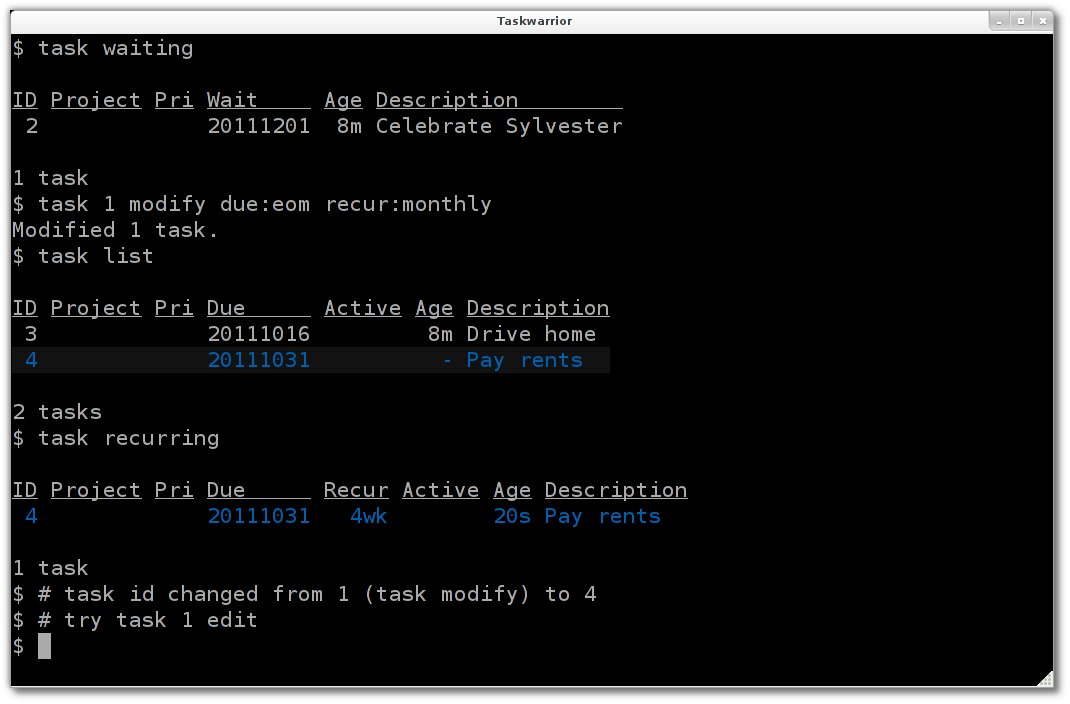
\includegraphics[width=10cm,height=7.5cm]{recur.png}
\end{center}
\end{frame}

\begin{frame}
\frametitle{Recurrence modifiers}
\begin{itemize}
\item hourly
\item daily, day, 1da, 2da, ...
\item weekdays
\item weekly, 1wk, 2wks, ...
\item biweekly, fortnight
\item monthly
\item quarterly, 1qtr, 2qtrs, ...
\item semiannual
\item annual, yearly, 1yr, 2yrs, ...
\item biannual, biyearly, 2yr
\end{itemize}
\end{frame}

\begin{frame}
\frametitle{Until and entry}
\begin{center}
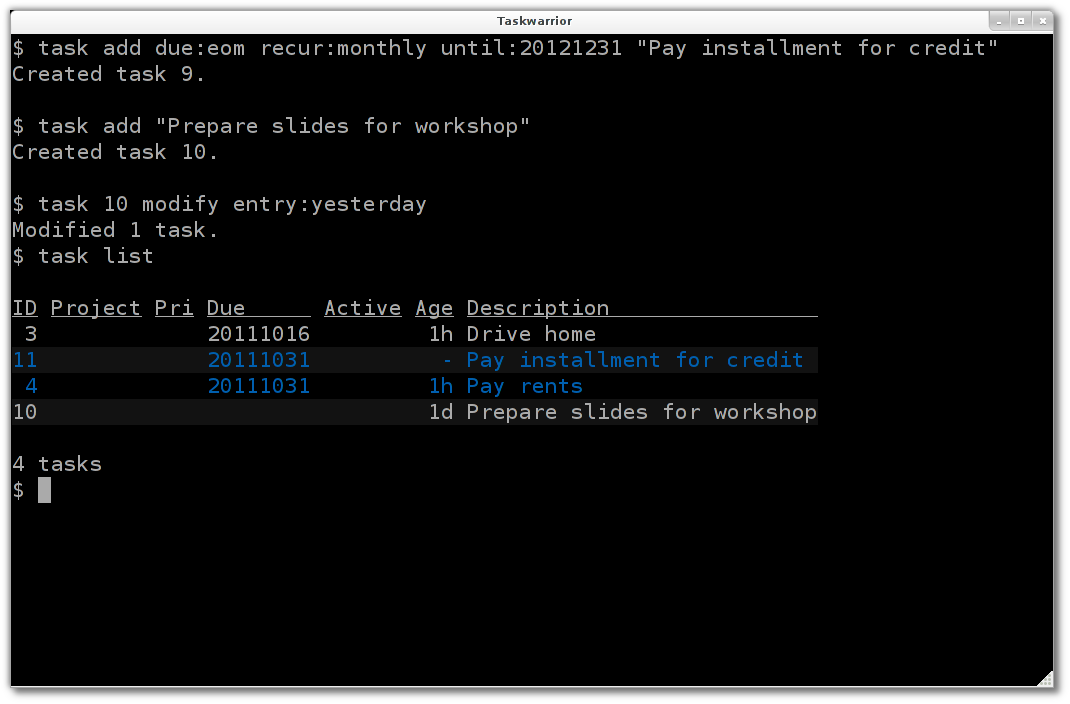
\includegraphics[width=10cm,height=7.5cm]{until_and_entry.png}
\end{center}
\end{frame}

\begin{frame}
\frametitle{Starting and stopping}
\begin{center}
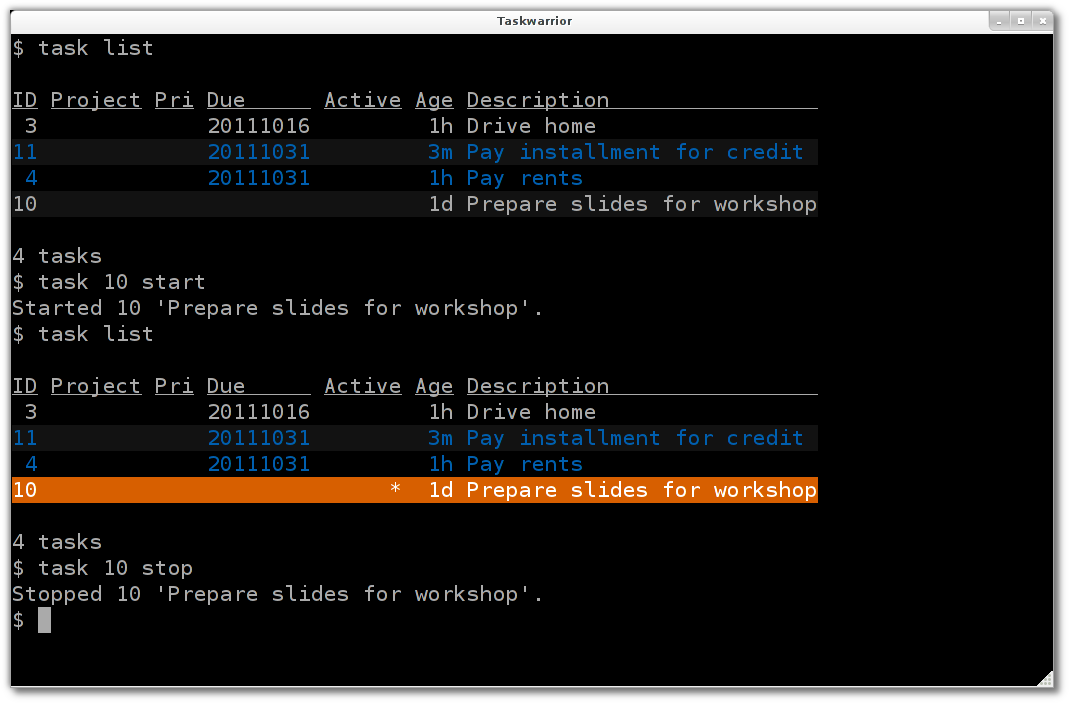
\includegraphics[width=10cm,height=7.5cm]{starting_and_stopping.png}
\end{center}
\end{frame}

\begin{frame}
\frametitle{Holiday}
\begin{alertblock}{Attention!}
Holiday has nothing in common with the German words "'Ferien"' or "'Urlaub"' (this would be vacation). (Public) Holiday means "'Feiertag"'.
\end{alertblock}

You can add holidays by either adding them via "'task config"' on the commandline or by adding them directly to the \textasciitilde/.taskrc-File or by including an external holiday definition.

On \href{http://holidata.net/}{holidata.net} you find a growing list of holiday dates, licensed CC-BY and offered by volunteers. Service was introduced by the Taskwarrior team, who is responsible for hosting and conversion to different formats.
\end{frame}

\begin{frame}
\frametitle{Add holiday}
\begin{center}
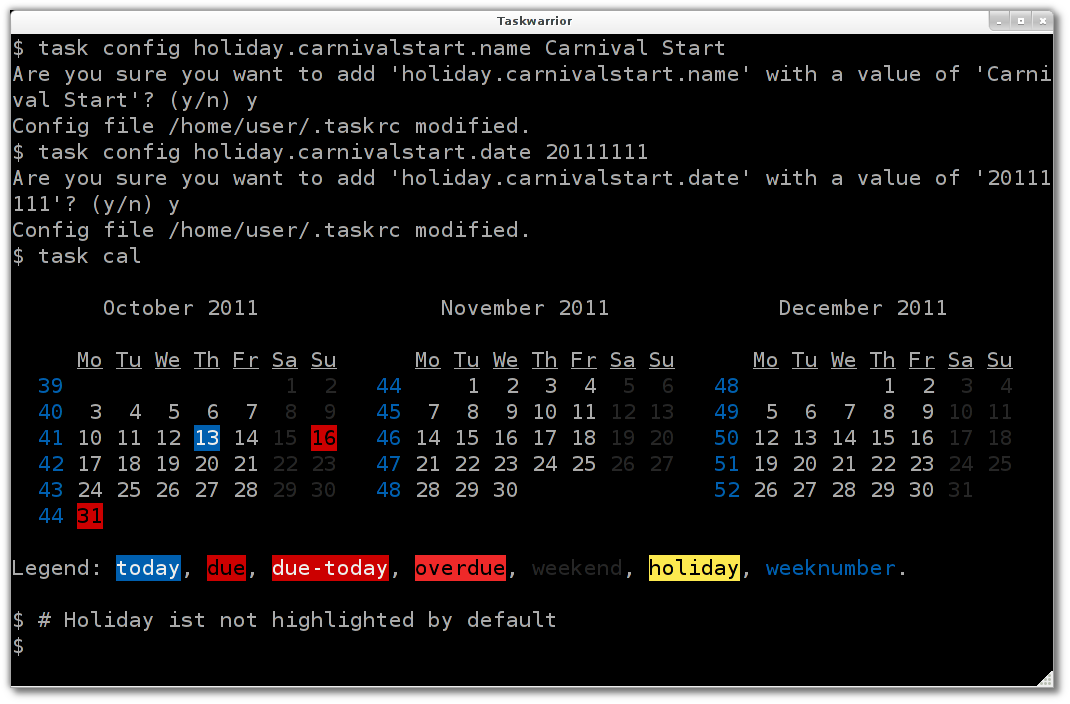
\includegraphics[width=10cm,height=7.5cm]{holiday_add.png}
\end{center}
\end{frame}

\begin{frame}
\frametitle{Calendar config with holiday}
\begin{center}
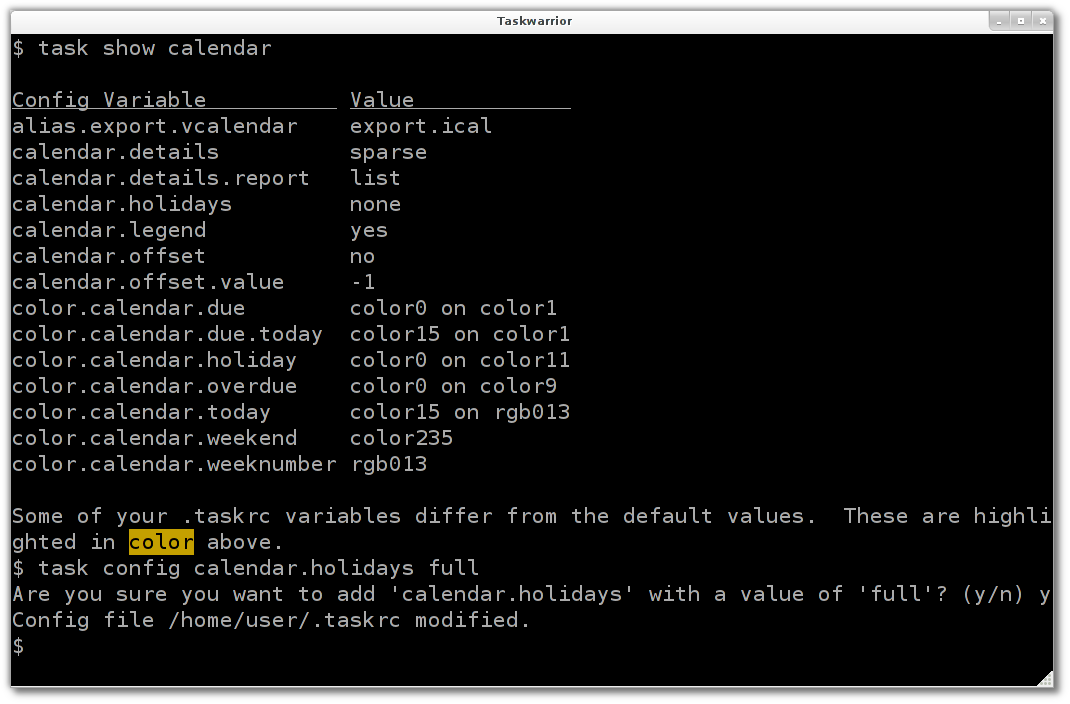
\includegraphics[width=10cm,height=7.5cm]{calendar_config_with_holiday_name.png}
\end{center}
\end{frame}

\begin{frame}
\frametitle{Calendar with holiday}
\begin{center}
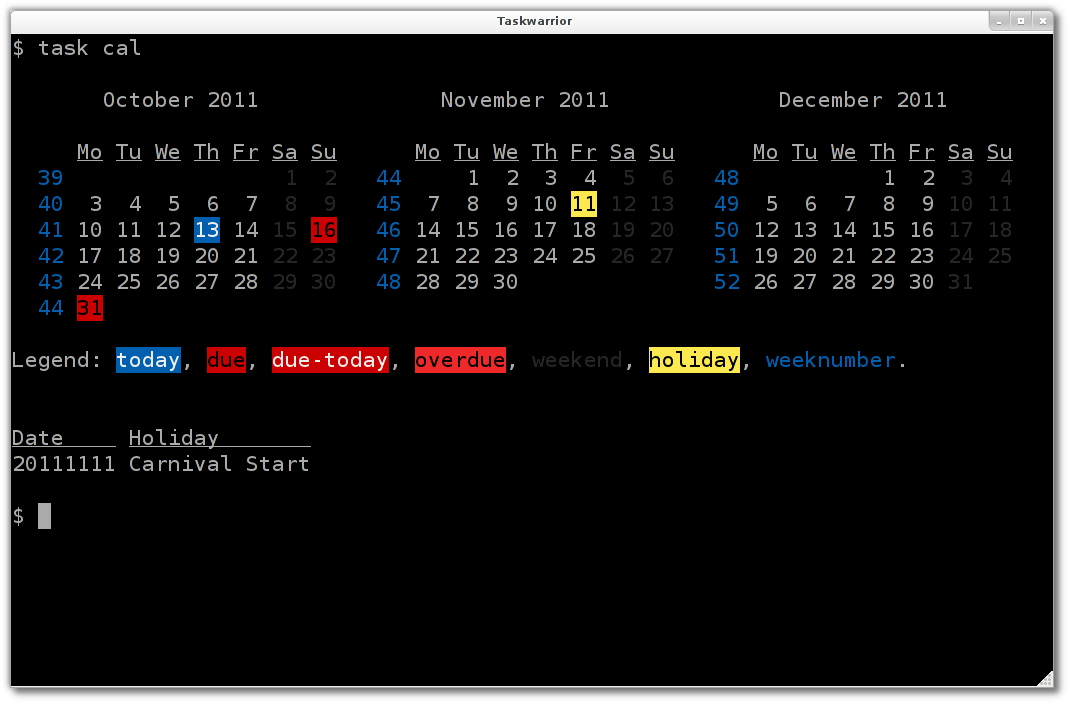
\includegraphics[width=10cm,height=7.5cm]{calendar_with_holiday_name.png}
\end{center}
\end{frame}

\begin{frame}
\frametitle{Calendar with due tasks}
\begin{center}
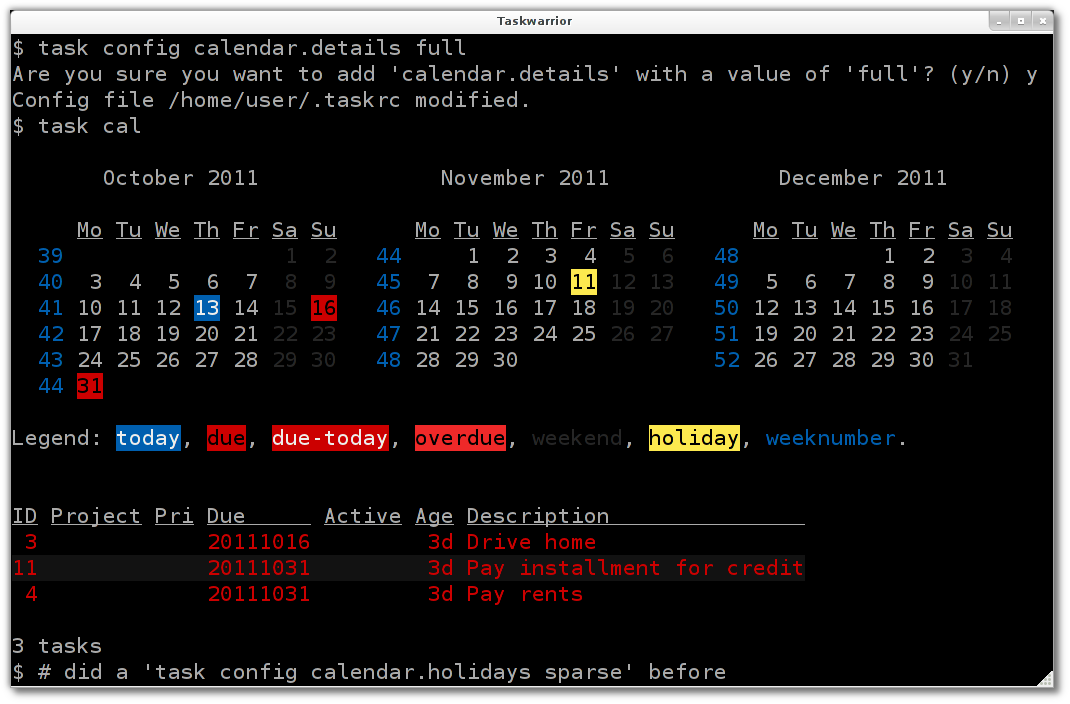
\includegraphics[width=10cm,height=7.5cm]{calendar_with_due_tasks.png}
\end{center}
\end{frame}

\section{Getting sorted}

\begin{frame}
\frametitle{Project and subproject}
\begin{center}
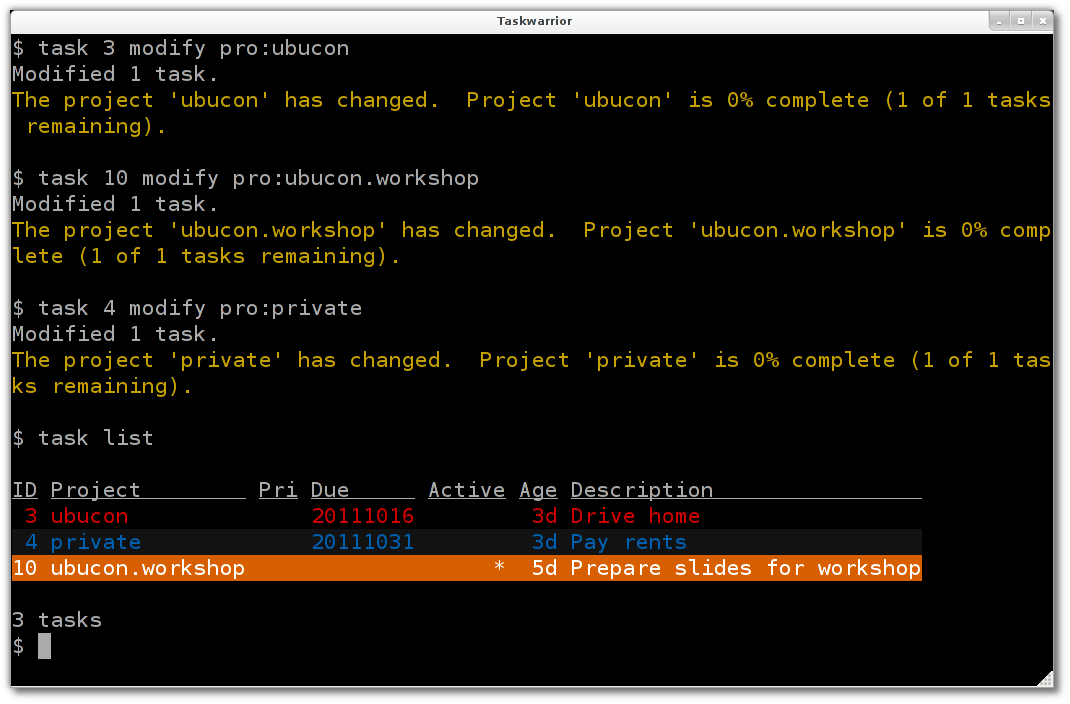
\includegraphics[width=10cm,height=7.5cm]{project_and_subproject.png}
\end{center}
\end{frame}

\begin{frame}
\frametitle{List of Projects}
\begin{center}
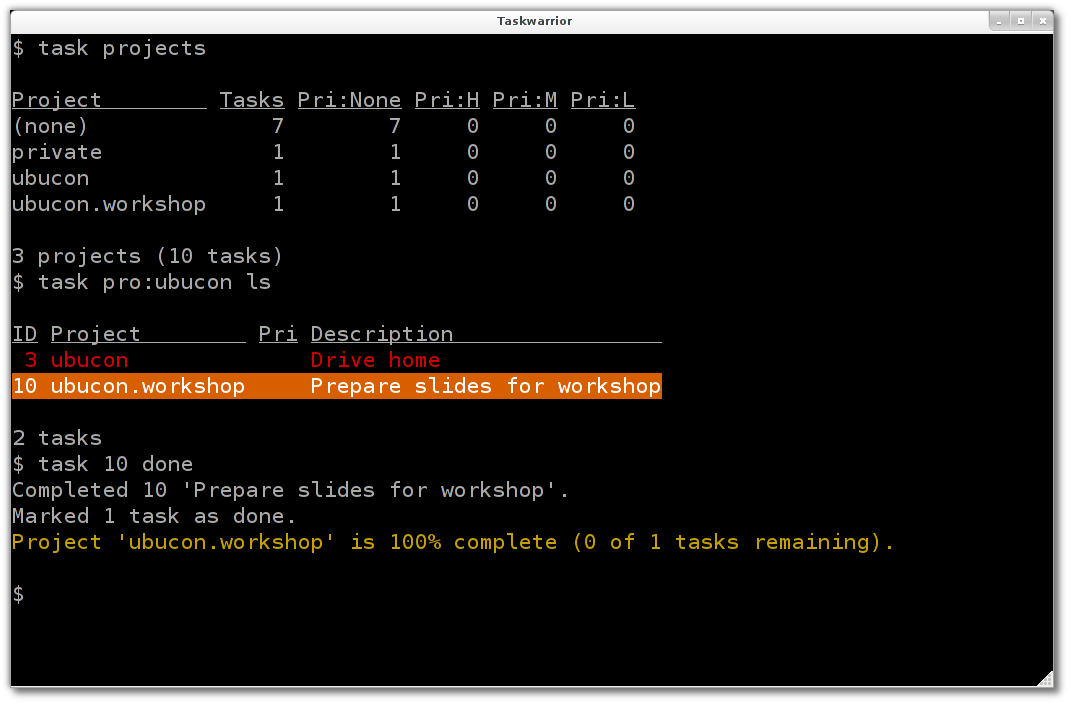
\includegraphics[width=10cm,height=7.5cm]{projects.png}
\end{center}
\end{frame}

\begin{frame}
\frametitle{Tags}
\begin{center}
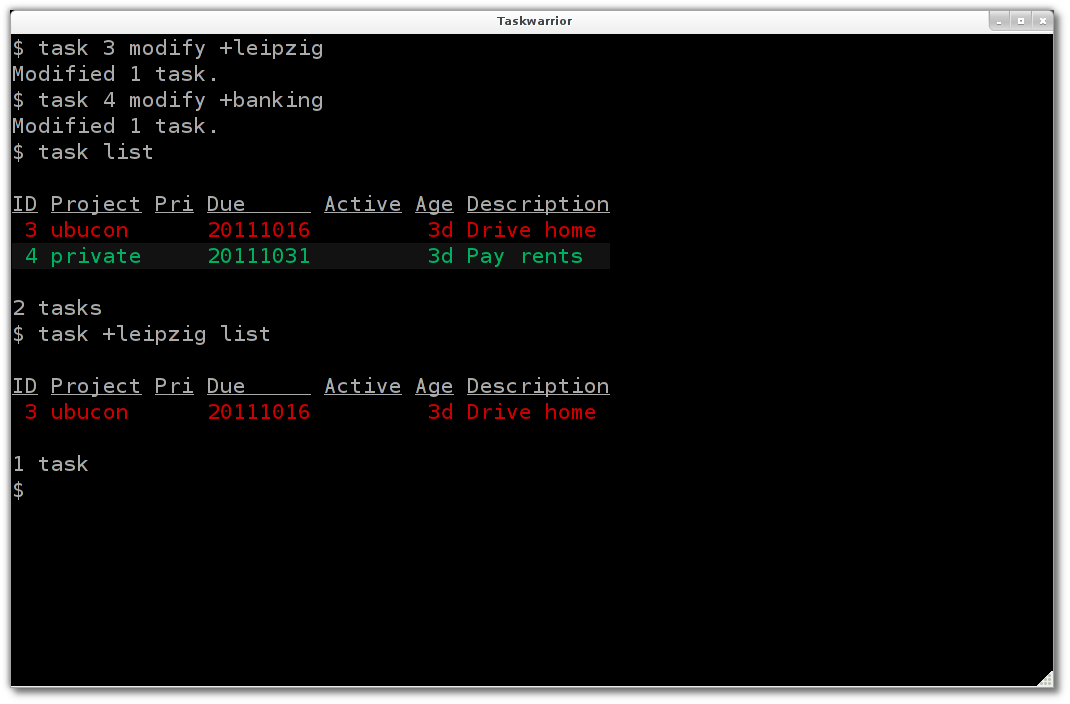
\includegraphics[width=10cm,height=7.5cm]{tags.png}
\end{center}
\end{frame}

\begin{frame}
\frametitle{Annotations}
\begin{center}
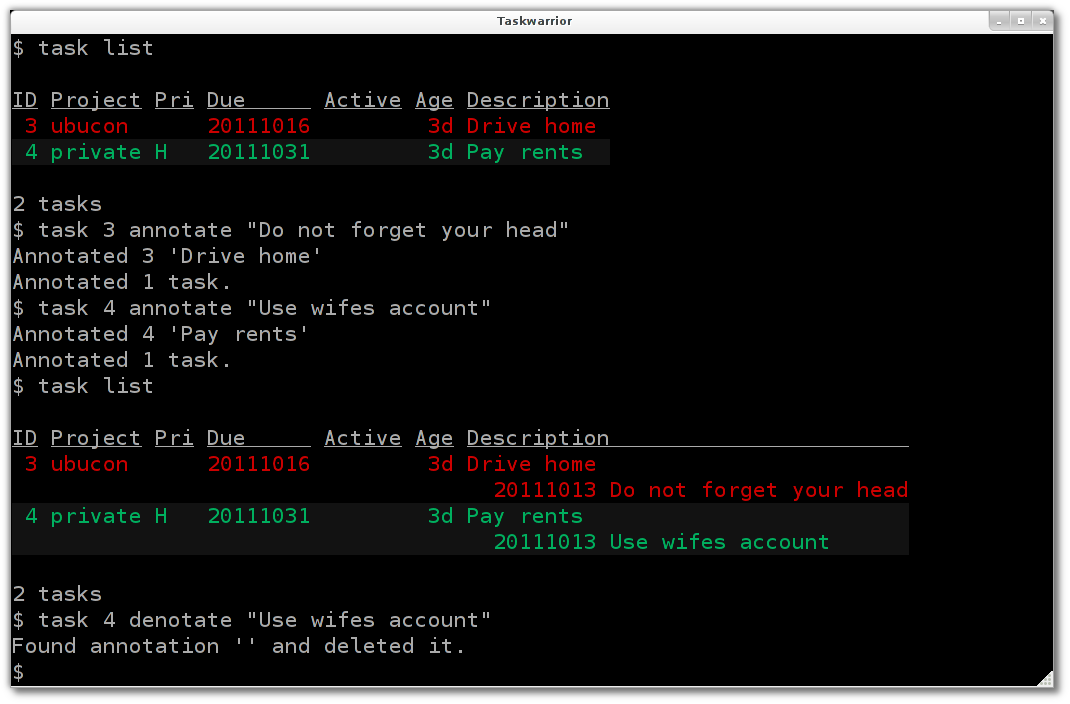
\includegraphics[width=10cm,height=7.5cm]{annotations.png}
\end{center}
\end{frame}

\section{Dependencies}

\begin{frame}
\frametitle{Dependency, part 1}
\begin{center}
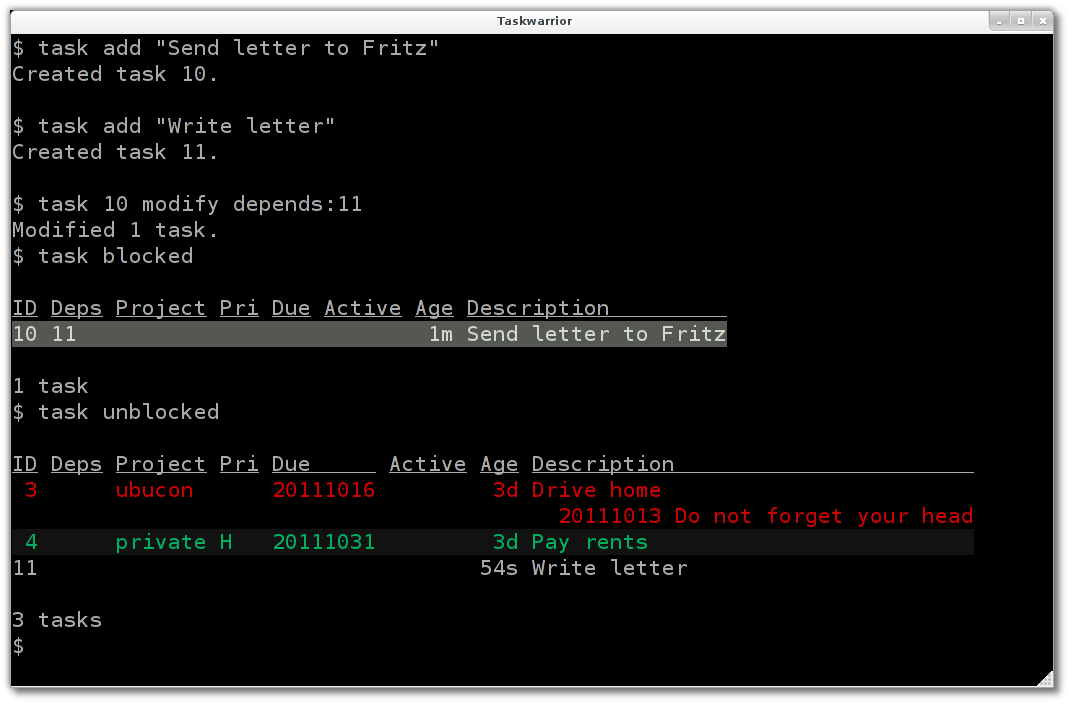
\includegraphics[width=10cm,height=7.5cm]{dependency01.png}
\end{center}
\end{frame}

\begin{frame}
\frametitle{Dependency, part 2}
\begin{center}
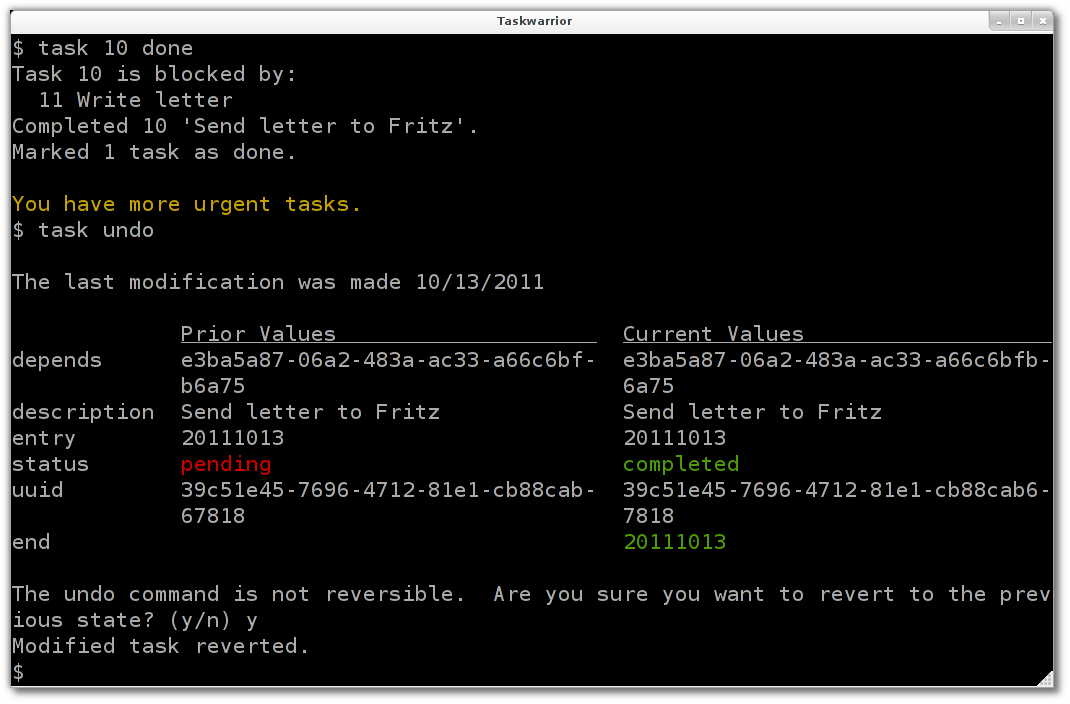
\includegraphics[width=10cm,height=7.5cm]{dependency02.png}
\end{center}
\end{frame}

\begin{frame}
\frametitle{Dependency, part 3}
\begin{center}
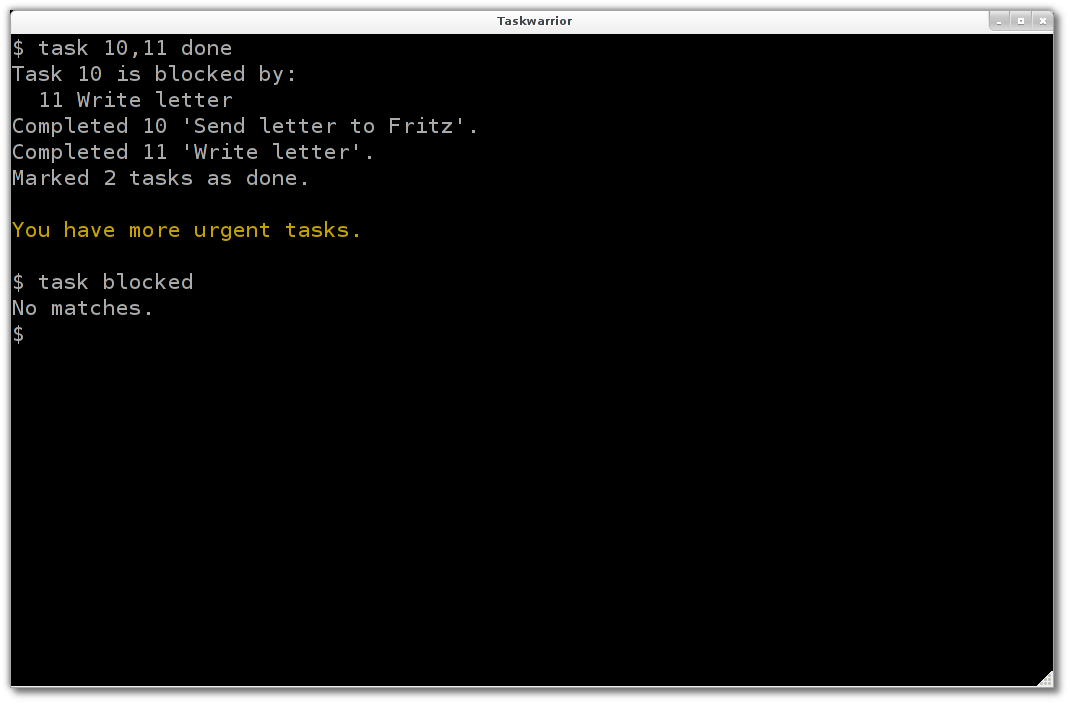
\includegraphics[width=10cm,height=7.5cm]{dependency03.png}
\end{center}
\end{frame}

\section{Reports}

\begin{frame}
\frametitle{Some predefined reports}

See \texttt{task reports} for a full list (26 reports).

\begin{itemize}
\item \textbf{active}           Lists active tasks matching the specified criteria
\item \textbf{all}              Lists all tasks matching the specified criteria, including parents of recurring tasks
\item \textbf{completed}        Lists completed tasks matching the specified criteria
\item \textbf{information}      Shows all data and metadata for specified tasks
\item \textbf{newest}           Shows the newest tasks
\item \textbf{next}             Lists the most urgent tasks
\item \textbf{oldest}           Shows the oldest tasks
\item \textbf{overdue}          Lists overdue tasks matching the specified criteria
\item \textbf{summary}          Shows a report of task status by project
\item \textbf{tags}             Shows a list of all tags used
\end{itemize}
\end{frame}

\begin{frame}
\frametitle{burndown.daily}
\begin{center}
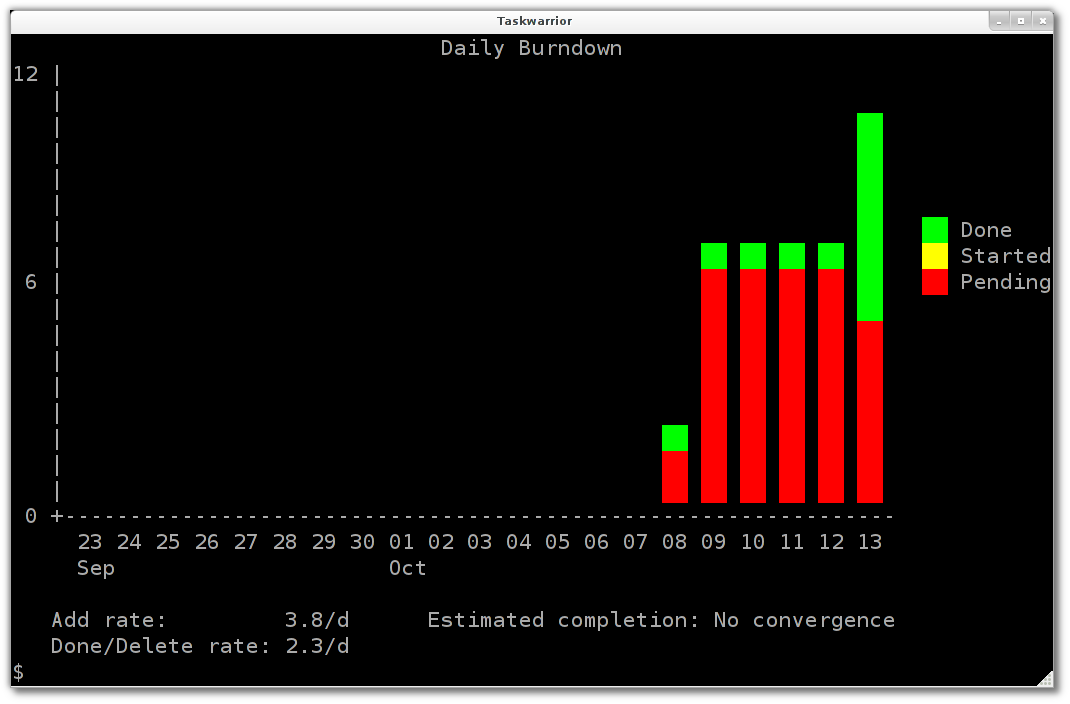
\includegraphics[width=10cm,height=7.5cm]{reports01.png}
\end{center}
\end{frame}

\begin{frame}
\frametitle{ghistory, history}
\begin{center}
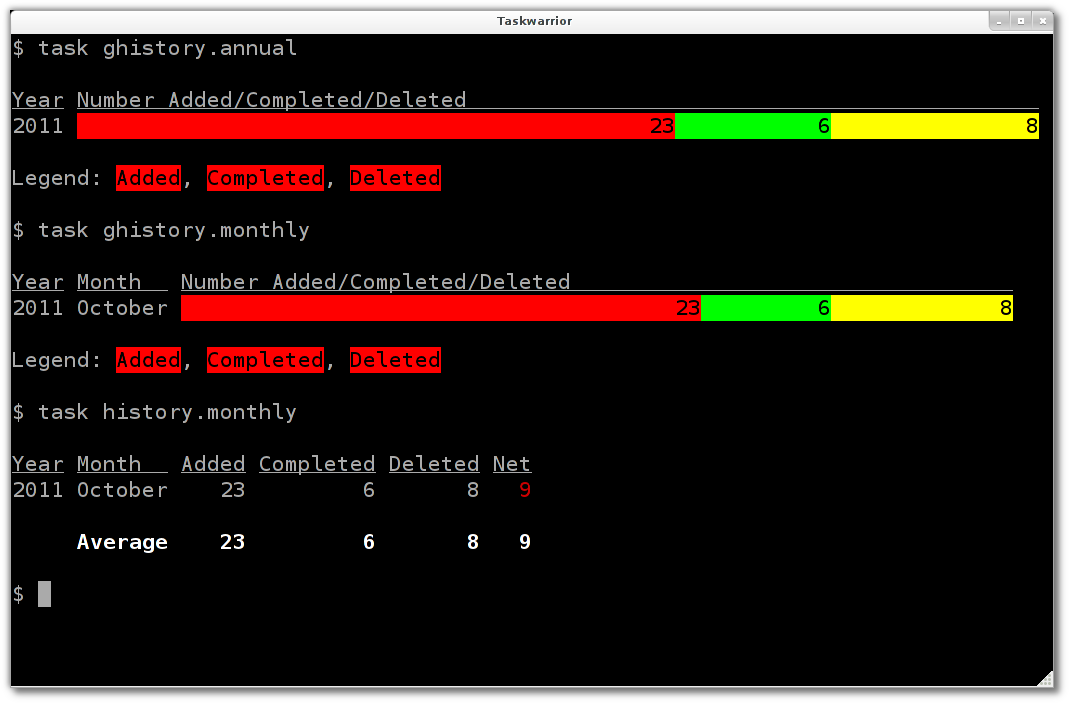
\includegraphics[width=10cm,height=7.5cm]{reports02.png}
\end{center}
\end{frame}

\begin{frame}
\frametitle{Report definitions}
\begin{center}
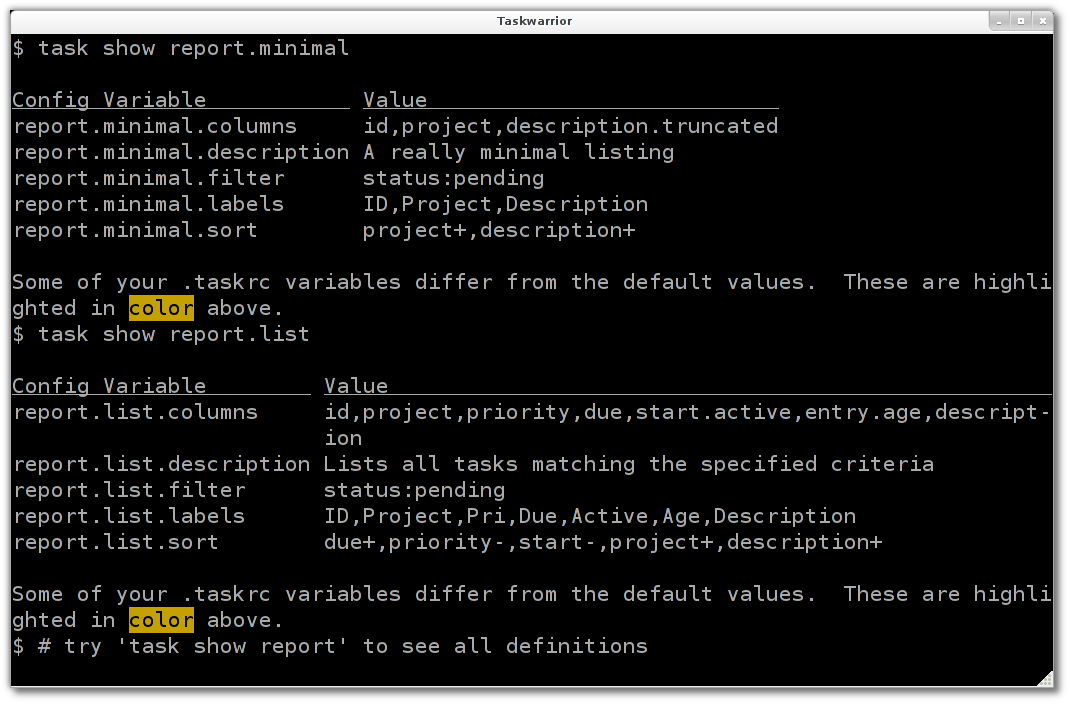
\includegraphics[width=10cm,height=7.5cm]{report_definitions.png}
\end{center}
\end{frame}

\begin{frame}
\frametitle{Dirks task list}
\begin{center}
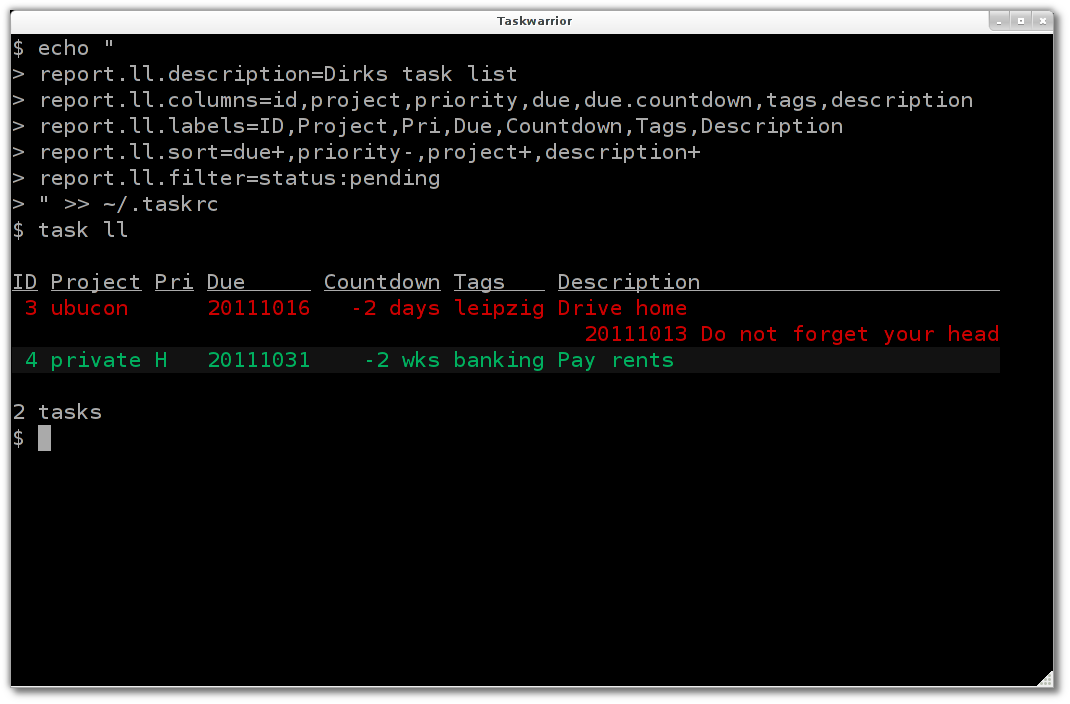
\includegraphics[width=10cm,height=7.5cm]{report_dirks_list.png}
\end{center}
\end{frame}

\begin{frame}
\frametitle{Set default command}
\begin{center}
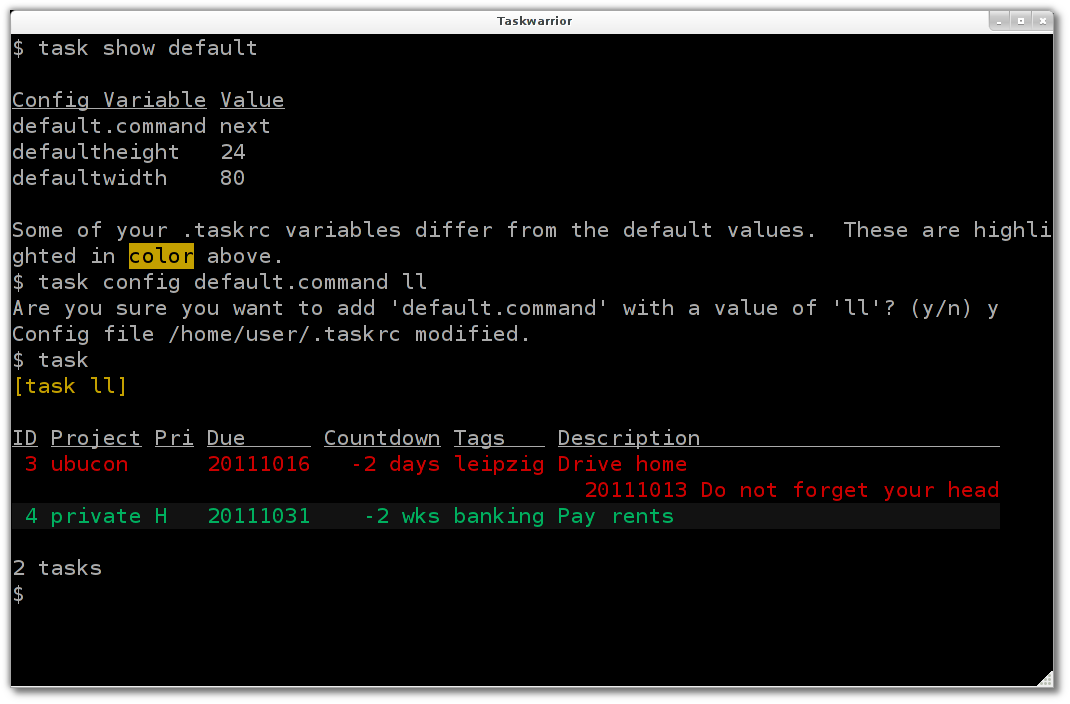
\includegraphics[width=10cm,height=7.5cm]{set_default_command.png}
\end{center}
\end{frame}

\section{Filtering}

\begin{frame}
\frametitle{Filtering in general}

You can filter for any modifier. If you don't use a modifier description is searched for the term, which may be a regular expression, on the command line. Filters may be combined.

The following attribute modifiers maybe applied as well. Names in brackets can be used alternatively.

So a filter can look like "'attribute.modifier:value"'.

\begin{itemize}
\item before, after
\item none, any
\item is (equals), isnt (not)
\item has (contains), hasnt
\item startswith (left), endswith (right)
\item word, noword
\end{itemize}
\end{frame}

\begin{frame}
\frametitle{Searches}
\begin{center}
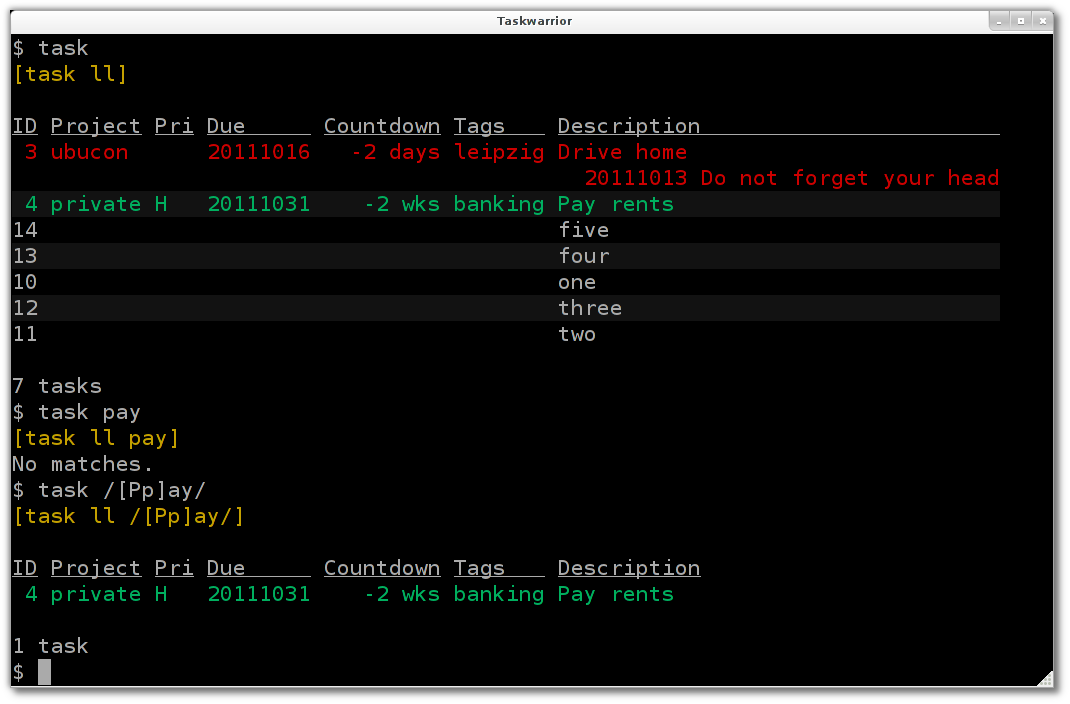
\includegraphics[width=10cm,height=7.5cm]{filter_searches.png}
\end{center}
\end{frame}

\begin{frame}
\frametitle{Attribute modifiers}
\begin{center}
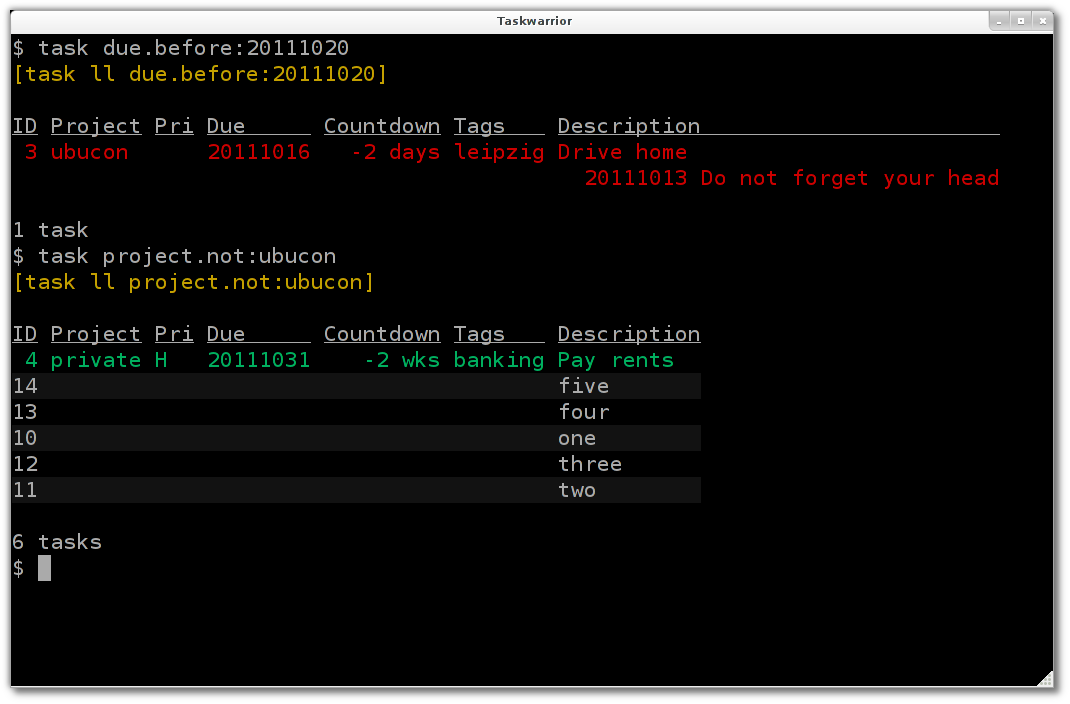
\includegraphics[width=10cm,height=7.5cm]{filter_attribute_modifiers.png}
\end{center}
\end{frame}

\begin{frame}
\frametitle{Combining}
\begin{center}
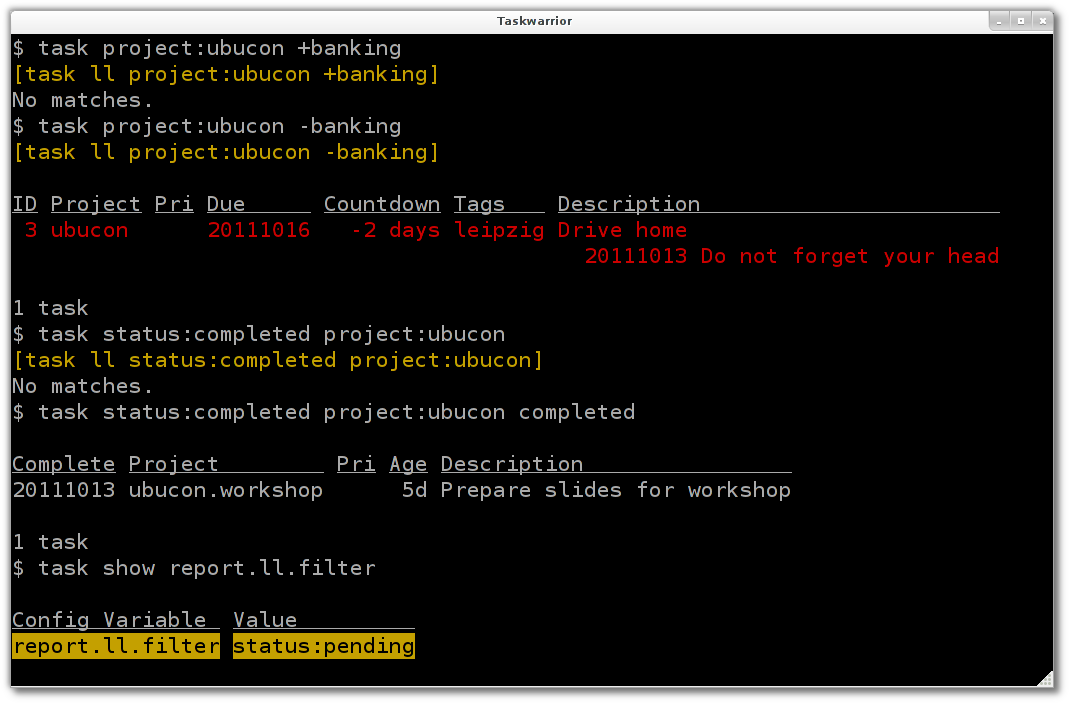
\includegraphics[width=10cm,height=7.5cm]{filter_combining.png}
\end{center}
\end{frame}

\section{That's all}

\begin{frame}
\frametitle{This is by far not all}
\begin{itemize}
\item \textbf{task log}  \\
for logging a task after it is already done.
\item \textbf{task diag} \\
to help support for diagnostic purpose.
\item \textbf{task shell} \\
a simple shell to get rid of the necessity to type "'task"' all the time.
\item ... and many more!
\end{itemize}
\end{frame}

\begin{frame}
\frametitle{Questions?}
\begin{center}

\includegraphics[width=6.4cm,height=7.5cm]{task_logo.png}
\end{center}
\end{frame}

\begin{frame}
\frametitle{Support}
\begin{center}
\href{http://taskwarrior.org/}{taskwarrior.org \\ 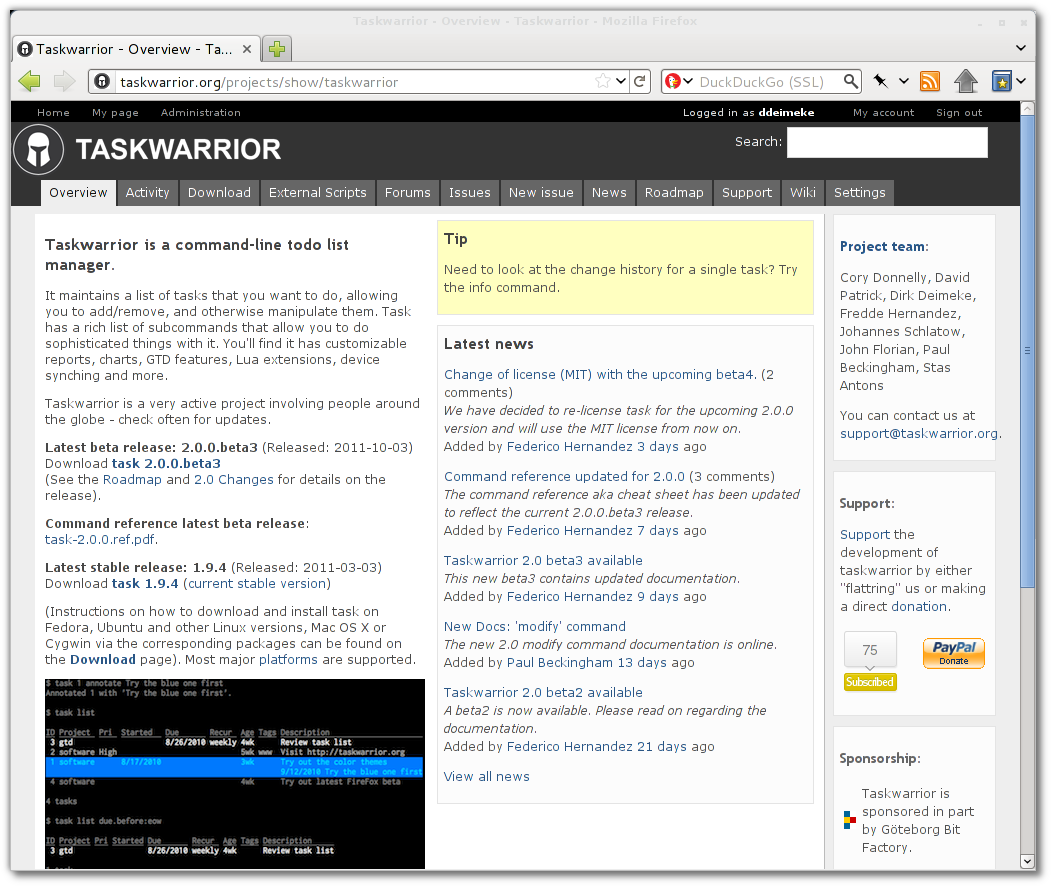
\includegraphics[width=8cm,height=6cm]{website.png}} \\
\href{mailto:support@taskwarrior.org}{support@taskwarrior.org} \\
\#taskwarrior on freenode.net -- @taskwarrior on Twitter or identi.ca
\end{center}
\end{frame}

\begin{frame}
\frametitle{Thanks for your patience!}
\begin{center}
Dirk Deimeke, Taskwarrior-Team, 2011, \href{https://creativecommons.org/licenses/by/3.0/}{CC-BY}

\href{mailto:dirk@deimeke.net}{dirk@deimeke.net}

\href{http://d5e.org/}{d5e.org} -- \href{http://dirk.deimeke.net/}{dirk.deimeke.net}
\end{center}
\end{frame}

\end{document}

%\begin{frame}[fragile]
%\frametitle{Title}
%\begin{lstlisting}
%\end{lstlisting}
%\end{frame}

%\begin{frame}
%\frametitle{title}
%\begin{center}
%\includegraphics[width=10cm,height=7.5cm]{name.png}
%\end{center}
%\end{frame}

%\begin{frame}
%\frametitle{title}
%\begin{itemize}
%\item \textbf{task {\tt<}filter{\tt>} modify}
%\end{itemize}
%\end{frame}

